\section{Zielsetzung}
    In diesem Versuch geht es um das Arbeiten mit Vakuum.
    Dabei werden die Drehschieberpumpe und die Turbomolekularpumpe genauer betrachtet.
    Das jeweilige Saugvermögen, sowie Leckatenmessungen werden durchgeführt und bestimmt.

\section{Theorie}
\label{sec:Theorie}
    Um die Arbeitsweise der Pumpen, sowie mögliche Probleme der Vakuumphysik zu verstehen wird zunächst auf die Grundlagen eingegangen.
    \subsection{Vakuum}
        Von einem Vakuum wird gesprochen, wenn der Druck in einem Raum niedrieger ist als $\SI{300}{\milli\BAR}$, also niedrieger als der geringste Atmosphärendruck auf der Erdoberfläche.
        Ab diesem Wert beginnt das sogenannte Grobvakuum und weitere Bereiche können defieniert werden.
        Je nach Druckbereich enstehen bestimmte Ströme, die auf die mittlere freie Weglänge der Gasteilchen zurückzuführen ist.
        Das liegt daran, dass mit abnehmender Teilchenzahldichte die mittlere freie Weglänge steigt.
        Diese Länge beschreibt den durchschnittlichen Abständen zwischen zwei Teilchenstößen. \\
        \noindent
        Im Grobvakuum ($\SIrange[]{300}{1}{\milli\BAR}$) herrschen vornehmend viskose Strömungen.
        Diese sind nochmals unterteilbar in laminare und turbolenter Strömung.
        Bei laminarer Strömung sind die mittleren freien Weglängen der Teilchen klein im Vergleich zu den Größen im Strömungskanal, sodass Stöße unter den Teilchen vorherrschen als mit den Wänden des Raumes.
        Dadurch bewegen sich die Teilchen in Bahnen, parallel zueinander.
        \noindent
        Das Feinvakuum beschreibt danach den Druckbereich von $\SIrange[]{300}{1e-4}{\milli\BAR}$.
        Hier sind Knudsenströmung auffindbar.
        Diese beschreiben den Übergang von viskoser zu molekularer Strömung.
        Die mittlere freie Weglänge ist hier in der Größenordnung des Strömungskanals.
        \noindent
        Der Bereich von $\SIrange[]{1e-3}{1e-7}{\milli\BAR}$ beschreibt das Hochvakuum, das Ultravakuum geht dann bis $\SI{1e-12}{\milli\BAR}$.
        Molekulare Strömung ist hier vertreten.
        Die mittlere freie Weglänge der Teilchen ist hier größer als die Abmessung des Strömungskanals, die Gasteilchen stoßen vermehrt gegen die Wände des Raumes als untereinander.
        \noindent
        Drücke, die kleiner als $\SI{1e-12}{\milli\BAR}$ sind, liegen im Bereich des extrem hohen Vakuums.
        \noindent
        In \autoref{fig:Strömung} ist eine Visualisierung der verschiedenen Strömungsarten und der mittleren freien Weglänge zu sehen.

        \begin{figure}
            \centering
            \includegraphics[width=\textwidth]{bilder/Strömung.png}
            \caption{Verscheidene Strömungsarten der Vakuumbereiche.\cite{Pfeiffer}}
            \label{fig:Strömung}
        \end{figure}

    \subsection{Ideales Gas und Druck}
        Im vorliegenden Versuch ist es ausreichend vom Modell des idealen Gases auszugehen.
        Hierbei wird angenommen, dass die Gasteilchen keine Ausdehnung haben und untereinander nur über vollkommen elastische Stöße wechselwirken.
        Dadurch kann das Gas mit der idealen Gasgleichung beschrieben werden:
        \begin{equation*}
            p \cdot V = N \cdot k_\text{B} \cdot T \, .
        \end{equation*}
        Hierbei beschreibt $p$ den Gasdruck, $V$ das Volumen des Raumes, $N$ die Teilchenzahl, $k_\text{B}$ die Boltzmann-Konstante und $T$ die Temperatur.
        Wird nun die Temperatur konstant gehalten, ist der Druck proportional zum Inversen des Volumens ($p \propto V^{-1}$).
        Dies ist auch unter das Gesetz von Boyle-Mariotte bekannt.
        \noindent
        Da der Druck die senkrechte Kraftkomponente auf eine Fläche beschreibt, gilt für die Einheit:
        \begin{equation*}
            \SI{1}{\newton\per\metre\square} = \SI{1}{\pascal} = \SI{1}{\milli\BAR} \, .
        \end{equation*}
        \noindent
        Zur Bestimmung des Saugvermögens $S$ wird das Gesetz von Boyle-Mariotte vewendet
        \begin{equation*}
            p \cdot V = \text{const}
        \end{equation*}
        und zeitlich abgeleitet.
        Dabei kann die zeitliche Ableitung des Volumens als Saugvermögen $S$ identifiziert werden:
        \begin{equation*}
            S = \frac{\text{d}V}{\text{d}t} = - \frac{V}{p} \frac{\text{d}p}{\text{d}t} \, .
        \end{equation*}
        Durch Lösen der DGL
        \begin{equation*}
            - \frac{S}{V} \cdot \dot{p} = p
        \end{equation*}
        mithilfe einer Exponentialfunktion entsteht ein Ausdruck für den Druck
        \begin{equation}
            p(t) = (p_0 - p_\text{E}) \cdot \exp{(- \frac{S}{V_0}t)} +p_\text{E} \, .
            \label{eqn:Druck_Funktion}
        \end{equation}
        Hierbei beschreibt $p_0$ den Anfangsdruck im Rezipienten und $p_\text{E}$ den Enddruck, den die Vakuumpumpe schließlich erzeugen kann.
        Durch die Aufnahme einer Evakuierungskurve kann das Saugvermögen mithilfe von \eqref{eqn:Druck_Funktion} ermittelt werden.

    \subsection{Sorption und Lecks}
        Um auf einige Herausfoderungen der Vakuumphysik einzugehen, muss es ein Verständnis von Sorption und Lecks geben.
        Allgemein beschreibt Sorption die Anreicherung eines Stoffes.
        Dabei wird noch unterschieden ob dieser Prozess innerhalb oder zwischen zwei Phasen abläuft.
        Das erste wird Absorption genannt, das zweite Adsorption.
        Entsprechend beschreibt die Desorption den Rückprozess.
        \noindent
        Lecks können das Vakuum verschlechtern.
        Auch hier gibt es eine Unterteilung zwischen realen und virtuellen Lecks.
        Die realen sind die Lecks, die Aufgrund des Versuchsaufbaus entstanden sind.
        Ein nicht richtig angschlossener Schlauch oder fehlende Dichtungen können reale Lecks sein und arbeiten somit gegen die Vakuumpumpe.
        Virtuelle Lecks entstehen z.B. bei der Produktion.
        Ein Beispiel wären Hohlräume, die bei der Produktion des Rezipienten oder ähnliches entstehen und sich beim Evakuieren öffnen.
        Kommt es zu Sorption im Evakuierungsprozess, kann das auch als virtuelles Leck beschrieben werden.
        Im Gegensatz zu realen Lecks können virtuelle schwer bis gar nicht gefunden oder im Nachhinein behoben werden.
        Als einzige Vorbeugungsmaßnahme von virtuellen Lecks muss in der Produktion der verschiedenen Teile so sauber wie möglich geabeitet werden.
        
        \subsubsection{Leckratenmessung}
            Die Leckrate $Q$ wird wie folgt definiert
            \begin{align*}
                S= \frac{Q}{p_\text{G}} \\
                \implies Q = V_0 \cdot \frac{\Delta p}{\Delta t} \, .
            \end{align*}
            $p_\text{G}$ beschreibt dabei den Gleichgewichtsdruck, $S$ das Saugvermögen.
            Somit entsteht auch ein Ausdruck für das Saugvermögen
            \begin{equation*}
                S = \frac{V_0}{p_G} \cdot \frac{\Delta p}{\Delta t} \, .
            \end{equation*}
            Werden nun mehrere Messungen mit unterschiedlichen Gleichgewichtsdrücken durchgeführt, so kann aus $\splitfrac{\Delta p}{\Delta t}$ das Saugvermögen $S$ bestimmt werden.

        \subsection{Leitwert}
            Da das effektive Saugvermögen $S_\text{eff}$, also das Saugvermögen, das letzendlich am Rezipienten ankommt, stark vom Aufbau der Vakuumanlage beeinflusst bzw. verringert wird, wird eine weitere Größe definiert.
            Der Leitwert $L$ beschreibt den sogenannten Strömungswiderstand, der durch Verbindungen wie Schläuche usw. verursacht wird.
            Somit wird das effektive Saugvermögen wie folgt ausgedrückt:
            \begin{equation*}
                S_\text{eff} = \frac{S_0 \cdot L}{S_0 + L} \, .
            \end{equation*}
            $S_0$ beschreibt dabei das theoretische Saugvermögen der Vakuumpumpe.


    \subsection{Vakuumerzeugung}
        Es gibt verschiedene Pumpen. Idk muss ich die verschiedenen Arten erklären? eig kB
        In diesem Versuch werden zwei Pumpen untersucht.
        Einmal die Drehschieberpumpe und die Turbomolekularpumpe.

        \subsubsection{Drehschieberpumpe}
            In \autoref{fig:Drehschieberpumpe} ist der schematische Aufbau einer Drehschieberpumpe zu sehen.
            Diese ist eine ölüberlagerte Rotationsverdrängerpumpe.
            Grob besteht die Pumpe aus zwei Ventilen, Ein- und Auslassventiel.
            Das Einlassventiel ist mit dem Rezipienten verbunden und schließt sich nicht.
            Das Auslassventiel dient dazu das Gas dann beim Pumpen in die Umgebung zu befördern, dazu kann das Ventiel geöffnet und geschlossen werden.
            Innerhalb des Gehäuses befindet sich der Arbeitsraum der Pumpe, worin ein Rotor und Schieber zu finden ist.
            Das Verhalten der Drehschieberpumpe kann auch mithilfe des Boyle-Mariotte-Gesetzes erklärt werden.
            Der Rotor läuft exzentrisch im Mittelpunkt des Arbeitsraumes, dabei wird ein größeres Volumen angeboten.
            Nach $p \cdot V = \text{const}$ fällt nun der Druck, da es einen Anstieg an Volumen gibt, in das auch die Gasteilchen gehen.
            Der Rotor dreht sich weiter und der mit Gas gefüllte Raum wird nun komprimiert.
            Das Volumen wird kleiner, der Druck somit größer.
            Sobald der Druck in diesem Raum den der Umgebung außerhalb der Pumpe übersteigt, wird das Auslassventil geöffnet und das Gas entweicht.
            So kann eine einstufige Pumpe einen Druck von $\SI{6e-2}{\milli\BAR}$ bis $\SI{6e-3}{\milli\BAR}$ im Rezipienten erzeugen.
            Zweistufige Drehschieberpumpen können einen Druck von $\SI{6e-4}{\milli\BAR}$ bis $\SI{6e-5}{\milli\BAR}$ erzeugen.
            In diesem Versuch wird eine einstufige Drehschieberpumpe verwendet.
      
        \begin{figure}[H]
            \centering
            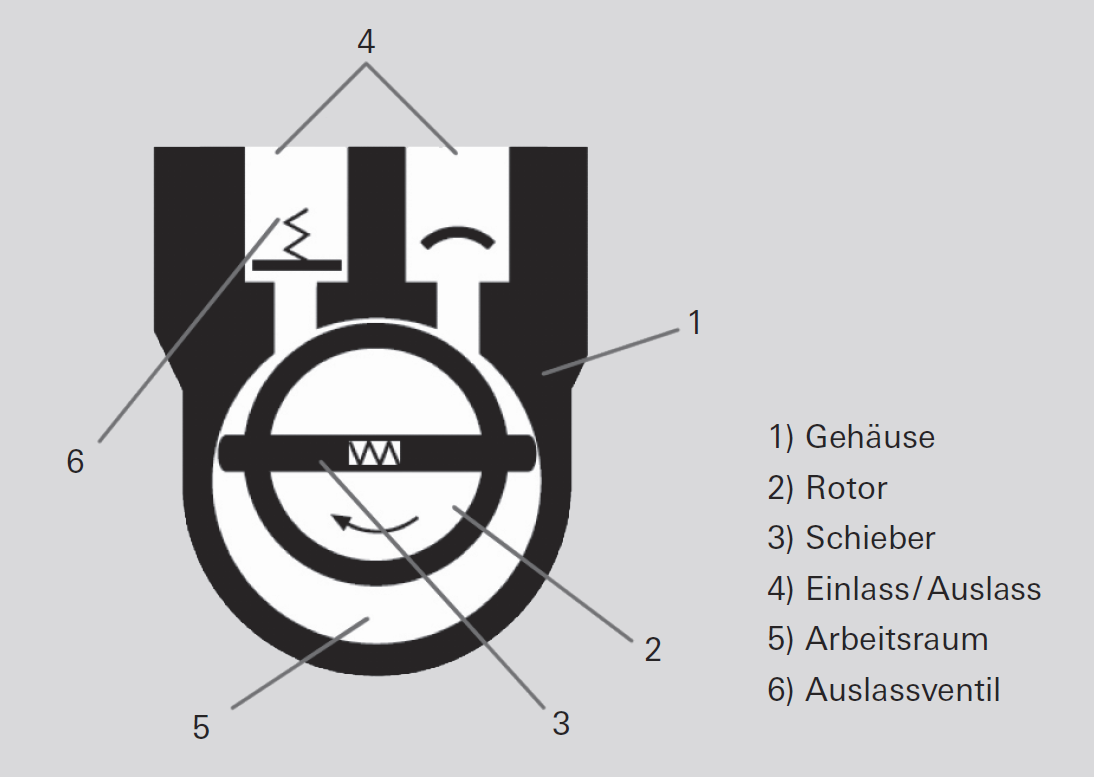
\includegraphics[width=\textwidth]{bilder/Drehschieberpumpe.png}
            \caption{Schematischer Aufbau einer Drehschieberpumpe.\cite{Pfeiffer}}
            \label{fig:Drehschieberpumpe}
        \end{figure}

        \subsubsection{Turbomolekularpumpe}
            Anders als die Drehschieberpumpe benötigt die Turbomolekularpumpe ein Vorvakuum um zu funktionieren.
            In \autoref{fig:Turbomolekularpumpe} ist eine Turbomolekularpumpe zu sehen.
            Im Inneren des Gehäusses sieht sie aus wie eine Turbine bzw. wie ein zusammengesetzte, mehrstufige Turbine.
            Dieser Rotor ist mit schaufelartigen Scheiben besetzt.
            Sie liegen schräg an.
            Ebenfalls sind weitere dieser Schaufeln spiegelverkehrt angebracht worden.
            Bei Drehung des Rotors werden die Gasteilechen durch Stöße mit den Rotorwänden in Pumprichtung beschleunigt.
            Damit das auch passiert, muss sich der Rotor mit einer Geschwindigkeit vergleichbar mit der der Gasteilche bewegen.
            Dafür dreht sich der Rotor dann mit einigen $\si{\kilo\hertz}$, bei der verwendeten Turbomolekularpumpe sind es $\SI{1350}{\kilo\hertz}$.
            So kann der Druck im Rezipienten schnell auf $\SI{1e-4}{\milli\BAR}$ gebracht werden.
            Weiter ist zu beachten, dass eine Turbomolekularpumpe selbst kein Vakuum erzeugen kann. 
            Sie muss mit einer weiteren Pumpe, z.B. mit einer Drehschieberpumpe zusammen eingesetzt werden.

        \begin{figure}[H]
            \centering
            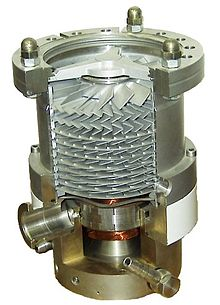
\includegraphics[width=\textwidth]{bilder/Turbomolekularpumpe}
            \caption{Das Modell einer Turbomolekularpumpe.\cite{turboBild}}
            \label{fig:Turbomolekularpumpe}
        \end{figure}

    \subsection{Vakuummessung}
        \subsubsection{Piezo-Vakuummeter}
            Das Piezo-Vakuummeter ist für die Messung im Grobvakuum geeignet.
            Die Idee dabei ist es die Kraft der Gasteilchen auf die Oberfläche gemessen.
            Das geschieht über ein Piezo-Kristall, der bei Kompression messbare elektrische Spannung erzeugt.

        \subsubsection{Pirani-Vakuummeter}
            Im Feinvakuum kann das Pirani-Vakuummeter verwendet werden, da hier die Wärmeleitfähigkeit proportional zum Druck ist.
            Ein stromdurchlossener Draht befindet sich im Rezipienten.
            Durch die Messung des Widerstandes des Leiters kann die Temperatur des Drahtes ermittelt werden.
            Der Draht kühlt sich dann abhängig vom Rezipienten-Druck unterschiedlich schnell ab, wodurch der Druck selbst bestimmbar ist.

        \subsubsection{Penning- und Bayard-Alpert-Vakuummeter}
            Beide Vakuummeter arbeiten im Hoch- und Ultrahochvakuum.
            Das Bayard-Alpert-Vakuummeter, ein Heiß-Ionisations-Vakuumeter arbeitet wie folgt:\\
            Elektronen werden durch thermische Emission freigesetzt.
            Diese werden zu einer Anode hin beschleunigt und können auf dem Weg Gasatome ionisieren.
            Diese ionisierten Gasatome werden zu einer Kathode beschleunigt, es ensteht ein Strom, der als Maß für die Vakuumqualität dient.
            \noindent
            Das Penning-Vakuummeter ist ein sogennantes Kalt-Ionisations-Vakuummeter.
            Bis auf die Elektronenerzeugung funktioniert dieses Vakuummeter genau wie das Bayard-Alpert-Vakuummeter.
            Hier werden die Elektronen durch elektrische Feldemission gewonnen.

        \noindent
        In diesem Versuch wird für die Vakuummessuug eine Kombination aus Piezo- und Pirani-Vakuummeter verwendet.
